\documentclass[twocolumn,10pt]{article}
\usepackage{ragged2e}
\usepackage{csquotes}
\usepackage{amsmath}
\usepackage{array}
\newcolumntype{C}{>$c<$}
\usepackage{mathtools}
%\usepackage{float}
\usepackage{hyperref}
\usepackage{amssymb}
\usepackage{amsthm}
\usepackage{bigints}
\usepackage{esvect}
\usepackage{pgfplots}
\usepackage{xcolor}
\usepackage{tikz}
\usepackage{multicol}
\usepackage{nonfloat}
\usepackage{wrapfig}
\newcommand*\circled[1]{\tikz[baseline=(char.base)]{
            \node[shape=circle,draw,inner sep=2pt] (char) {#1};}}
\usepackage{textcomp}
\RequirePackage{color,graphicx}
\usepackage{graphicx,subcaption}
\usepackage{caption}
\usepackage[paper=letterpaper,margin=0.8in]{geometry}
\newcommand\myeq{\stackrel{\mathclap{\normalfont\mbox{L'H}}}{=}}
\definecolor{amaranth}{rgb}{0.9, 0.17, 0.31}
\usepackage[noabbrev,capitalise]{cleveref}
\usepackage{titlesec}

\DeclareRobustCommand{\abbrevcrefs}{%
\crefname{figure}{fig.}{figs.}%
\crefname{equation}{eqn.}{eqns.}%
%\crefname{table}{tbl.}%
}

\DeclareRobustCommand{\cshref}[1]{{\abbrevcrefs\cref{#1}}}

%custom figure code for multicol
\makeatletter
\newenvironment{tablehere}
  {\def\@captype{table}}
  {}

\newenvironment{figurehere}
  {\def\@captype{figure}}
  {}
  
\newenvironment{subfigurehere}
  {\def\@captype{subfloat}}
  {}
\makeatother

\begin{document}

\onecolumn
%---------Put name and information on the top right-----------%
\centering{\huge Assignment 2}\\~\\

%\null\hfill\begin{tabular}[t]{l@{}}
%\textbf{Hammad Ahmed Sheikh}\\
%\textsc{hshammads@csu.fullerton.edu}\\
\textsc{cpsc 488: natural language processing}\\
\textsc{10/14/2024}\\
\textsc{dr. christopher ryu}\\
\textsc{california state university, fullerton (CSUF)}\\~\\
%\textsc{November 5, 2023}\\~\\~\\
%\end{tabular}

%---------body of the pitch-----------%
\begin{multicols}{2}
\begin{flushleft}
\justifying

\section*{Assignment Information}
This assignment can be completed individually or by a team with up to 5 members.\\
Total score: 100\\
Due date: 10/31/2024 11:59PM\\
Members: Hammad Sheikh, Matthew Do, Ryan Avancena \\
Work distribution: Equal

\iffalse
\subsection*{Objectives}
In this exercise, you will learn how to develop a sentiment analysis model and an an automated trading system relying on the analysis results.
\textcolor{blue}{Only Python programs written using Python 3.0 or higher will be accepted}. \textcolor{red}{NO Jupyter notebook or any other Python variants} will be accepted for efficient grading.\\

$\hrulefill$
\subsection*{About the dataset and problem to solve}
A stock, in investment terms, represents ownership in a company. When you buy stocks, you essentially buy a small piece of that company. The stock price for a company is mainly determined by the current value of the company that can be computed by the company’s past financial data (e.g., earnings, revenues, profits, etc.) and future value determined by the company’s future performance, which is unknown. The intrinsic value of a company refers to the actual and inherent worth of the company based on both current and future value. Therefore, a stock price is determined by the current value and estimated (perceived) future value of the company. Investors buy stocks based on the company’s estimated intrinsic value. That’s why the stock prices inherently fluctuate depending on the market situation and the company’s future prospectus, which are typically published in news articles. The more information investors have, the better they can estimate the intrinsic value.
\textbf{Tesla} may be one of the companies that generate the most news articles due to their market impact and technological innovations. In this assignment, you will analyze the Tesla stock (the stock symbol, \textbf{TSLA}) price data and related news articles to develop a simple trading system. Your trading system will be equipped with a sentiment analysis model that analyzes all the (directly or indirectly) Tesla-related news articles for about 10 years, computes its market impact, and trades only TSLA based on the impact. For example, your trading system will buy a certain number of shares if the news article is considered positive and the balance is enough to cover the trade. Otherwise, the system will sell a certain number of shares if the news article is negative and a sufficient number of shares are already owned. The \textcolor{green}{ultimate goal} is maximizing the \textcolor{green}{return} from the initial investment, utilizing the sentiment analysis model.

\subsection*{Required activities}
\textcolor{red}{\textbf{Utilize} the \textbf{GPU} resources available on the \textbf{Nautilus} through the \textbf{Kubernetes}} for modeling (\textbf{NOT} by the JupyterHub) and \textcolor{red}{\textbf{write} an analysis report} about your system's modeling results and trading performance by answering all the questions below with your \textbf{\textcolor{red}{justification} supported \textcolor{red}{by the data}}.

\begin{enumerate}
	\item \textbf{Download} the historical price data for TSLA and its (directly or indirectly) related news articles between 1/1/2013 to the last market closing date (today or yesterday) from any free data sources (e.g., Yahoo Finance) and save the data in a JSON file format on your local machine. JSON is an open standard file format used for data storage or exchange. The price data should include market date, open price, high price, low price, closing price, and volume. The news articles may be related to the entire market, not necessarily only to TSLA. The direct TSLA-related news can be articles about the company that you can download from the data source. Examples of indirect TSLA-related news can be the news about the market (Dow Jones \^DJI, S\&P \^GSPC, Nasdaq \^IXIC, or the industry Tesla belongs to). Briefly describe the types of news articles you downloaded for your system, explaining why and how you downloaded the data.
	
	\item \textbf{Develop} a sentiment analysis model using Multilayer Perceptron (MLP) that can quantitatively estimate the impact of each news article on the TSLA price. Briefly describe 
		\subitem (a) The methods used to (pre)process the news and price data for your MLP algorithm with justification and 
		\subitem (b) the method(s) used to analyze the news and quantify its impact that will be used for trade.
	
	\item \textbf{Backtest} your trading system based on the sentiment analysis model developed in (2) and measure its performance. Backtesting means testing the effectiveness of trading systems that utilize specific trading algorithms. In this case, your sentiment analysis model is a trading algorithm. For the backtesting, assume your account has an initial investment balance of \$100,000, and buy/sell orders will always be filled without trading fees. 

	To evaluate the performance of your trading algorithm, you need to \textbf{develop a simple trading system} that will buy a certain number of TSLA shares only if the balance is sufficient to cover the purchase and the positive market impact computed by the model or sell a certain number of shares only if it already holds enough number of shares (\textcolor{red}{no short sell allowed}) and the negative market impact. 
	\textbf{Evaluate your system’s trading performance} \underline{so far} by calculating the following simple metrics\\
		\subitem (a) \$gain or \$loss for each trade, 
		\subitem (b) the total $gain or $loss for all trades, 
		\subitem (c) \% return compared to the initial balance. 
		
	\textbf{Log every trade}, including the key transaction data such as\\
		\subitem (a) the transaction date, 
		\subitem (b) trading type buy/sell, 
		\subitem (c) \# of shares traded, 
		\subitem (d) \$amount used for the trade, and 
		\subitem (e) the current balance after the trade to a log file \enquote{\textcolor{purple}{trade\_log.json}} for future analysis, verification, or accounting purpose.
		
	\textbf{Display the trading summary}, including the 
		\subitem (a) total \$gain or \$loss for all trades and
		\subitem (b) \% return compared to the initial balance (\$100,000.00).

	\item \textbf{Briefly describe} at least two methods or techniques (based on the relevant topics discussed in class) to improve the model performance and evaluation results on whether or not those methods improved the trading performance.
	
	\item \textbf{Create word embeddings} based on Word2vec, other embedding method, or pre-trained embedding for your model and compare the trading performance with the best model without relying on word embeddings.
\end{enumerate}

\textcolor{red}{\textbf{Warning:}} Although you can reuse any source codes available on the Internet, you are not allowed to share your codes with any other team or students in this class. Any student or team violating this policy will receive a \textbf{ZERO} score for this assignment, potentially for all the remaining assignments.

\subsection*{What to submit}
\begin{itemize}
	\item \textcolor{blue}{One analysis report} includes \textcolor{blue}{all your member names}, \% contribution made by each member, and all the answers to the questions based on your analysis in \textbf{PDF} or \textbf{Word format}. If every member contributed equally, simply state \enquote{\textcolor{purple}{equal contribution}.} If your team does not agree on individual contributions, briefly write a task description for each member. Different grades may be assigned based on individual contributions, even if a group completed the work.
	
	\item \textbf{Upload one analysis report file} and \textbf{Python program file(s)}, individually. Please \textcolor{red}{DO NOT upload any zip file} since Canvas cannot open it.
	
	\item When you show some example data in your analysis report (when necessary), select only a few examples, not including the entire dataset.
	
	\item Submit only one for each team.
\end{itemize}

\subsection*{Grading criteria}
\begin{itemize}
	\item The overall quality of work shown in the report about modeling results, supporting data, analysis process, methods used, and correctly implemented programs
	\item The level of understanding as reflected in the report
	\item Effort (10\%)
\end{itemize}
\fi

$\hrulefill$

\textit{Abstract} - Machine learning (ML) and Artificial Intelligence (AI) worlds are experiences tremendous growth. Their applications are uncountable. One realm of applications for ML and AI is Natural Language Processing (NLP). In this aspect, there are various classification
models that assist with text classification and processing. Our goal for this assignment is to utilize NLP techniques in analyzing news data for Tesla to build a ML model that would maximize our investment returns. The stock data can be obtained via the Python libraries that Dr. Ryu \cite{cryu} defined. News articles will be scraped from the web.\\
\textit{Keywords} - Stock Trading, Tesla, Natural Language Processing, Machine Learning

	\tableofcontents
	
	\section{Introduction} \label{introduction}
	There is a lot of stock data available in the world. All the stocks are impacted by the environment and the economical status of the world. This information is shared via news articles, which are in text format. We need to able to analyze news data, identify patterns and sentiment, and utilize it to predict impact on stocks. However, due to the sheer size of data available and the amount of convolution, it is not an easy task for a human. If we can
utilize the computing power and technology available in computers, we may be able to make an impact. This may not have been possible a few decades ago. However, with the expansion of ML and AI technologies, numerous applications become available. With the use of NLP, we can perform text classification and sentiment analysis.\\
	Without generalizing too much, let us look at a specific stock, Tesla (ticker TSLA), with the goal of applying existing text classification and sentiment analysis algorithms on news and stock data, and analyzing their results for performance and accuracy to maximize our investment returns. 
	
	\section{Approach} \label{approach}
	The generalized approach is shown below in \cref{fig:gen_approach}. (Data Acquisition $\rightarrow$ Data Pre-Processing $\rightarrow$ Data Classification and Sentiment Analysis $\rightarrow$ Model Development for Investment $\leftrightarrow$ Parameter and Feature Adjustment to Maximize Investment Returns.) Further details will be discussed in the following sections. 

	\begin{figurehere}
		\centering
		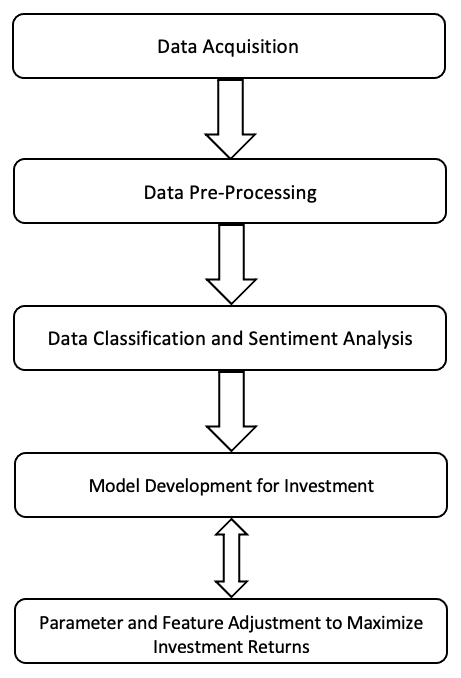
\includegraphics[width=0.65\linewidth]{images/gen_approach.png}
		\caption{Generalized Approach}
		\label{fig:gen_approach}
	\end{figurehere}
	
	\mbox{}\\
	We will be relying on existing libraries as much as possible. This will help to focus on the classification and sentiment analysis task instead of building code from scratch for things that already exist. For example, train\_test\_split from sklearn.model\_selection \cite{scdatasplit} will be utilized to split the data into training and testing datasets.
		
	\subsection{Data Acquisition} \label{data_acquisition}
	%\textit{\underline{Note from Dr. Ryu:}} You can use any package to download the data, but some popular Python packages may be \textbf{yfinance} or \textbf{yahoo-fin} or \textbf{both}. You \textbf{don't want} to use \textbf{rudimentary approaches like web scrapping as it will take too long time, and you are not sure about the data quality.}\\
	The first step in data processing, regardless of whether it is for our assignment or any other project, is data acquisition. We need to have a dataset that can be used to train need based models.\\
	Our assignment needs two main datasets; one for stock information and one for news articles. For the TSLA stock information, we utilized Python library yfinance \cite{yfin} to download the data and stored it locally in JSON files. For the news articles, we (\textcolor{red}{NEED TO FILL IN THIS INFORMATION}). This enables us to have a defined set of data, which we can preprocess and utilize in our model development of sentiment analysis and investment returns.\\
	
	\cref{fig:tsla_hist} shows a sample snapshot of TSLA market data acquired from yfinance \cite{yfin}.
	
	\begin{figurehere}
		\centering
		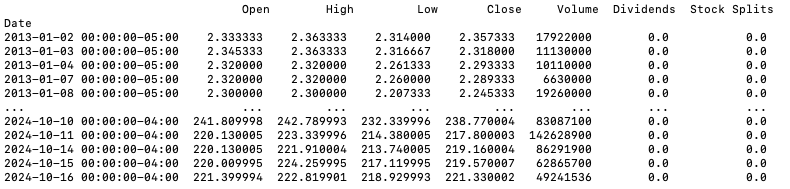
\includegraphics[width=\linewidth]{images/tsla_hist.png}
		\caption{Sample snapshot of TSLA market data}
		\label{fig:tsla_hist}
	\end{figurehere}
	
	\subsection{Data Pre-Processing} \label{data_preprocessing}
			
	\subsection{Data Classification and Sentiment Analysis} \label{class_model_analysis}
	
	\mbox{}\\
	\begin{tablehere}
		\centering
		\resizebox{\columnwidth}{!}{%
		\begin{tabular}{C|C|C|C|C|C}
			\text{Model/Evaluation Metric} & \text{Accuracy} & \text{Sensitivity or Recall} & \text{Specificity} & \text{Precision} & \text{Harmonic mean}\\
			\hline
			\text{Bernoulli Naïve Bayes} & 86.18\% & 21.89\% & 94.88\% & 36.65\% & 27.41\%\\
			\text{Logistic Regression} & 88.30\% & 17.63\% & 97.87\% & 52.78\% & 26.43\%\\
			\text{Default MLP} & 88.74\% & 41.56\% & 94.55\% & 50.79\% & 45.71\%\\
			\text{Adjusted MLP} & 90.05\% & 34.14\% & 97.61\% & 65.95\% & 44.99\%			
		\end{tabular}
		}
		\caption{Classifiers' Evaluation Metrics}
		\label{tab:classevalmetrics}
	\end{tablehere}

	\subsection{Model Development for Investment} \label{investment_model_dev}
	
	\subsection{Parameter and Feature Adjustment to Maximize Investment Returns} \label{adjustment_models}
	
	
	
	\section{Conclusion and Future Work} \label{conclusion}
		
	
	\section{Acknowledgements} \label{acknowledgements}
	I would like to acknowledge Dr. Jin \cite{rjin} for ML, classification and probability distribution concepts, Professor Avery \cite{avery} for MLP concepts, 

\bibliographystyle{IEEEtran}
\bibliography{references}

\end{flushleft}
\end{multicols}
\end{document}